%%%%%%%%%%%%%%%%%%%%%%% file template.tex %%%%%%%%%%%%%%%%%%%%%%%%%
%
% This is a general template file for the LaTeX package SVJour3
% for Springer journals.          Springer Heidelberg 2010/09/16
%
% Copy it to a new file with a new name and use it as the basis
% for your article. Delete % signs as needed.
%
% This template includes a few options for different layouts and
% content for various journals. Please consult a previous issue of
% your journal as needed.
%
%%%%%%%%%%%%%%%%%%%%%%%%%%%%%%%%%%%%%%%%%%%%%%%%%%%%%%%%%%%%%%%%%%%
%
% First comes an example EPS file -- just ignore it and
% proceed on the \documentclass line
% your LaTeX will extract the file if required
\begin{filecontents*}{example.eps}
%!PS-Adobe-3.0 EPSF-3.0
%%BoundingBox: 19 19 221 221
%%CreationDate: Mon Sep 29 1997
%%Creator: programmed by hand (JK)
%%EndComments
gsave
newpath
  20 20 moveto
  20 220 lineto
  220 220 lineto
  220 20 lineto
closepath
2 setlinewidth
gsave
  .4 setgray fill
grestore
stroke
grestore
\end{filecontents*}
%
\RequirePackage{fix-cm}
%
%\documentclass{svjour3}                     % onecolumn (standard format)
%\documentclass[smallcondensed]{svjour3}     % onecolumn (ditto)
\documentclass[smallextended]{svjour3}       % onecolumn (second format)
%\documentclass[twocolumn]{svjour3}          % twocolumn
%
\smartqed  % flush right qed marks, e.g. at end of proof
%
\usepackage{graphicx}
\usepackage{amsmath}
\usepackage{amsfonts}
\usepackage{caption}
\usepackage{subcaption}
\usepackage{hyperref}
\captionsetup{compatibility=false}
%
% \usepackage{mathptmx}      % use Times fonts if available on your TeX system
%
% insert here the call for the packages your document requires
%\usepackage{latexsym}
% etc.
%
% please place your own definitions here and don't use \def but
% \newcommand{}{} 
%
% Insert the name of "your journal" with
% \journalname{myjournal}
%
\begin{document}

\title{Comparison of Mixed Integer Programming Formulations for the Shared Multicast Tree Problem%\thanks{Grants or other notes
%about the article that should go on the front page should be
%placed here. General acknowledgments should be placed at the end of the article.}
}
\subtitle{Tightening the LP bounds}

%\titlerunning{Short form of title}        % if too long for running head

\author{Marika Ivanova        \and
         Dag Haugland%etc.
}

%\authorrunning{Short form of author list} % if too long for running head

\institute{F. Author \at
              first address \\
              Tel.: +123-45-678910\\
              Fax: +123-45-678910\\
              \email{fauthor@example.com}           %  \\
%             \emph{Present address:} of F. Author  %  if needed
           \and
           S. Author \at
              second address
}

\date{Received: date / Accepted: date}
% The correct dates will be entered by the editor


\maketitle

\begin{abstract}
In this paper we focus on the Shared Multicast Tree problem (SMT), which is 
a task in wireless network design aiming to establish a wireless 
communication network minimizing necessary energy consumption. SMT is a 
generalization of the Shared Broadcast Tree problem (SBT), and can be 
regarded as a Steiner tree problem with a nonlinear objective functinon that
reflects the use in wireless communication. In particular, we consider two 
integer linear programming formulations and investigate how they relate to 
each other. The first model extends the original SMT model, while the second one 
is based on a strong formulation of the minimum Steiner tree problem. In 
addition, we present several valid inequalities. Our goal is to achieve a 
stronger LP bound than models studied in previous works, and also to devise 
a method which allows calculating these lower bounds for instances as 
large as possible. Numerical experiments suggest that both models are much 
stronger than previous formulations, however, the number of constraints 
makes them impractical for solving instances of even fairly small size as 
the computation takes prohibitively long time. Applying a constraint 
generation scheme on one of the studied models significantly increases the 
size of the instances for which it is possible to obtain a strong LP 
bound. 
\keywords{Wireless communication, broadcast tree, multicast, Steiner tree, LP bound, 
valid inequalities}
% \PACS{PACS code1 \and PACS code2 \and more}
% \subclass{MSC code1 \and MSC code2 \and more}
\end{abstract}

\section{Introduction}

\label{intro}

The purpose of a multicast communication in a wireless ad-hoc network is to route information from a sending device to a set of receiving devices. Given a set of wireless devices and distances between them, the task is to assign power to each device, so that the demands of the communication are met and the energy consumption is as low as possible, assuming their locations are fixed. Power efficiency is an important measure in designing ad-hoc wireless networks since the devices typically use batteries as power supply and are therefore heavily energy-constrained. Individual devices work as transceivers, which means that they have the ability to both transmit and receive a signal. Moreover, the power level of a device can be dynamically adjusted during a multicast session.

Unlike wired networks, nodes in ad-hoc wireless networks use omnidirectional antennas, and hence a message reaches all nodes within the communication range of its sender. This range is determined by the power assigned to the sender, which is the maximum rather than the sum of the powers necessary to reach all intended receivers. This feature is often referred to as the wireless multicast advantage \cite{Wieseltier00onthe}. 

A well known and extensively studied task in wireless network design is the Minimum Energy Broadcast (MEB) problem. Given a set of wireless devices with one designated source node among them, the goal is to assign power to individual nodes  which determines their communication ranges, inducing a broadcast tree such that a signal initiated by the source reaches all the remaining nodes, and the energy consumption for this communication is minimized. Typically, not only one node can act as a source. Every node may initiate a message intended for the remaining nodes. In general, two different sources have two different optimal broadcast trees, which means that the optimal broadcast trees must be calculated separately for every node. Furthermore, in order to route signals correctly, the nodes must be able to recognize which node initiated currently received signal and therefore which broadcast tree is used, or from the relaying device's perspective, which power level should be set. It is obvious that such overhead calculations require additional energy and certain abilities of used devices.

The idea of the SBT problem is to maintain a single broadcast tree regardless the source of a signal. Such tree would not be optimal for individual sources, but routing at each node would be considerably simplified. Provided that a single broadcast tree is used, the nodes are no longer required to identify the source of the message in order to set a correct power level. Instead, only the immediate neighbour from which the signal was received must be recognized. The objective function in SBT captures not only the power levels of the nodes, but depends also on how often a node actually transmits using certain power level. A natural extension of this concept and a forefront of this paper is the Shared Multicast Tree (SMT) problem, in which some of the nodes never initiate any transmission and do not have to receive any signals. They can be used as intermediate forwarding nodes whenever it reduces the resulting power, and thus play the role of Steiner nodes. Devices that can initiate a transmission and also have to receive every message are referred to as \emph{destinations}.

\subsection{Related work}
\subsection{Assumptions and notation}
An ad-hoc wireless network is modeled by a complete graph $G=(V,E)$, where the set $V$ of nodes represents the set of wireless devices and the set of edges $E=\{\{i,j\}:i,j\in V, i\neq j\}$ corresponds to the potential links between them. Often we use the set $A=\{(i,j):i,j\in V,\{i,j\}\in E\}$ that contains all arcs derived from $E$. The set $D\subseteq V$ of \emph{destinations} denotes selected devices that initiate a communication and also are required to receive every message initiated by some other destination. The remaining devices represented by $V\setminus D$ do not have to receive the messages, but can be used as an intermediate nodes and relay a transmission whenever it reduces energy consumption. Next, $d: V\times V\rightarrow \mathbb{R}$ is a function that determines a distance between every two nodes. The constant $\alpha$ represents an environmentally dependent parameter typically valued between 2 and 4. Power requirement $p_{ij}$ for sending a message from node $i$ to $j$ is then calculated as $p_{ij}=d^{\alpha}_{ij}$, implying the symmetry $p_{ij}=p_{ji}$. The task is to find a Steiner tree minimizing given objective function explained in the next section.

If $\{i,j\}$ is an edge in a Steiner tree $T=(V_T,E_T)$ of $G$, we use $T_{i/j}$ to denote the subtree of $T$ consisting of all vertices $k$ such that the path from $k$ to $j$ visits $i$, as introduced in \cite{Haugland12Dual}. Additionally, we define a function $\text{nod}(T_{i/j})$ that returns the number of destinations in $T_{i/j}$. Neighbours of $i$ in $T$ are denoted $i^T_1$, $i^T_2$, $i^T_3, \dots$ in non-increasing order of distance from $i$. If there is no risk of confusion, we simply omit the superscript $T$. The highest and second highest power levels of $i$ are defined by its neighbours $i_1$ and $i_2$, respectively. For a leaf $i$, we set $p_{ii_2}=0$.

Let $\mathbf{z} \in \{0,1\}^E$ be a binary vector with components corresponding to edges in $E$. The undirected graph induced by $\mathbf{z}$ is defined as  $G_\mathbf{z}=(V,E_\mathbf{z})$, where $\{i,j\}\in E_\mathbf{z}\Leftrightarrow x_{ij}=1$. The directed graph induced by $\mathbf{x} \in \{0,1\}^A$ is defined analogously. In both cases, the induced (directed) graph is not necessarily connected. If A is an IP model, its continuous relaxation is denoted as A-LP.

The reminder of this paper is organized as follows: Section \ref{sec:SBT} describes the SMT problem and gives detailed explanation of its objective function. Integer linear programming formulations, valid inequalities and their analysis are presented in Section \ref{sec:ILP}. Results of various numerical experiments are reported in Section \ref{sec:exp}, followed by conclusions in Section \ref{sec:conclusion}.
\section{Shared Broadcast and Multicast Tree problem}
\label{sec:SBT}

A feasible solution to an SMT instance is any Steiner tree for given set of destinations $D$ in $G$. Assume the tree $T=(V_T, E_T)$ depicted in Fig. \ref{fig:objexp} to be one such solution. Any node $s\in D$ can initiate a transmission, and all the remaining destinations must receive it. Let us now consider the node $i$ with three neighbours $i_1$, $i_2$ and $i_3$ ordered downwards by their distance from $i$. If the transmitting node is $a$, $b$ or $i_1$, then the signal reaches $i$ via arc $(i_1,i)$ and all nodes in the subtree $T_{i_1/i}$ highlighted by the grey area have already received the signal, and so $i$ does not have to send it back to $i_1$. It suffices if $i$ forwards the signal to the most distant neighbour different than $i_1$, which is in our case $i_2$. By using the power level $p_{ii_2}$ and due to the wireless advantage, the message reaches all the neighbours that have not received it yet. On the other hand, if the transmission is initiated by a destination from $T\setminus T_{i_1i}$ (outside the grey area), then $i$ has to forward it to the most distant neighbour $i_1$, which again causes that all nodes that have not received the signal will be reached.
\begin{figure}[h!]
        \centering
        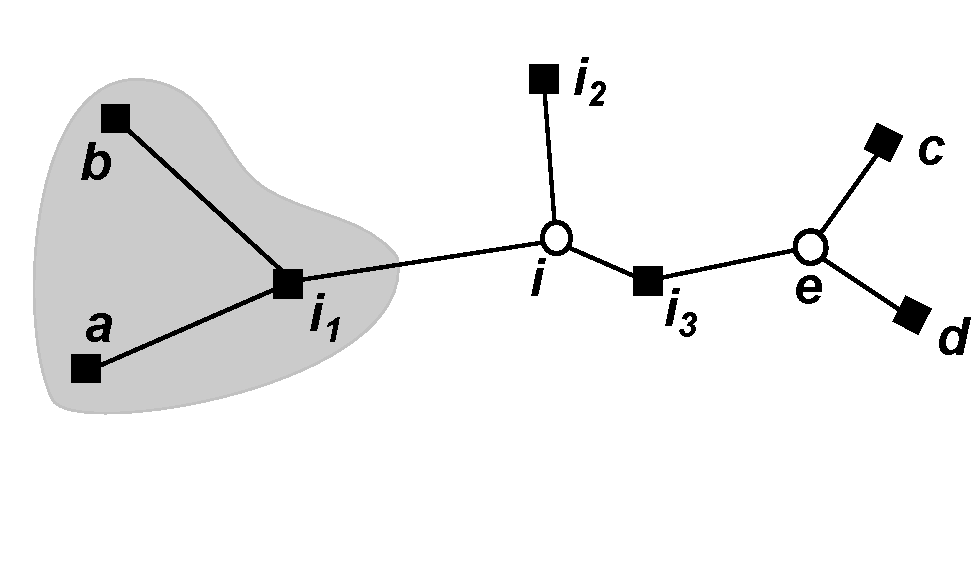
\includegraphics[height=1.6in]{objexp}
        \caption{A simple feasible solution illustrating the calculation of a contribution of node $i$ to the objective function. Destinations and Steiner nodes are denoted by solid squares and empty circles, respectively.}
                \label{fig:objexp}
\end{figure}

 The non-linear objective function captures the entire network structure and takes account of frequency of usage of certain power level. In our example, node $i$ uses the power level $p_{ii_2}$ every time the source of the relayed signal lies in the subtree $T_{i_1/i}$ which contains three potential sources. The power level $P_{ii_1}$ is set whenever the source lies outside of $T_{i_1/i}$, which applies to four sources. The contribution of node $i$ to the objective function is thus $3p_{ii_2} + 4p_{ii_1}$. The total cost of $T$ is the sum over all nodes' contributions. In general,
$$
c(T) = \sum\limits_{i\in V_T}\left[nod(T_{i_1/i})p_{ii_2} + nod(T\setminus T_{i_1/i})p_{ii_1}\right].
$$ 

Like most of the wireless network design problems presented in literature, SBT/SMT is NP-hard \cite{Haugland11Compact}.

\section{MIP Formulations}
\label{sec:ILP}

In this section, we state MIP formulations of the SMT problem, explain function of individual constraints, and analyse relations between them. A basic element of every MIP formulation for SMT is a set of constraints modelling a Steiner tree. We investigate two such Steiner tree models and draw a comparison  between them. Both models have variables of at most 3 indices, and are further extended and strengthened by 4-index variables.
\subsection{Original SMT Model [SMTO]}
The first model we consider is slightly improved SMT model introduced in \cite{ivanova16isco} which contains a weaker version of constraint (\ref{con:dd:arrowFromNonDestA}). This model extends the SBT formulation from \cite{Haugland12Dual} by the Steiner nodes in order to formulate the multicast version of the problem. The model uses three sets of binary variables defined as follows:
\newline\newline
  $z_{ij}=
	\begin{cases}
    1 & \text{if edge $\{i,j\} \in E$ is in the solution},\\
    0 & \text{otherwise},
  \end{cases}$
\newline\newline
  $x^{s}_{ij}=
	\begin{cases}
    1 & \text{if arc $(i,j) \in A$ is used to transmit a message from $s\in D$},\\
    0 & \text{otherwise}.
  \end{cases}$
  \newline\newline
  $y^s_{ij}=
	\begin{cases}
    1 & \text{if node $i \in V$ uses power $p_{ij}$ to transmit a message from $s\in D$},\\
    0 & \text{otherwise}.
  \end{cases}$
\newline
\newline    
\begin{subequations}
\begin{flalign}
\label{objective:dd} &\makebox[0pt][l]{$\displaystyle{}\min \sum\limits_{(i,j) \in A} \sum\limits_{s \in D} p_{ij} y^s_{ij} $}  & &&\\ \notag  
\text{s.t.}&  &  &                 && \\	\
\label{con:dd:maxsize}\sum\limits_{\{i,j\}\in E}z_{ij} & \leq  N-1 &  && \\
\label{con:dd:arrowFromDest} \sum\limits_{j\in V_i}x^s_{ji} & = 1 && i,s\in D,i\neq s && \\ 
\label{con:dd:arrowFromNonDestB} \sum\limits_{j\in V_{i}}x^s_{ji} & \leq 1 && i\in V \setminus D, s\in D   &&\\	
\label{con:dd:arrowFromNonDestA} x^s_{ik}  & \leq \sum\limits_{j\in V_{i}\setminus \{k\}}x^s_{ji} && i\in V \setminus D,(i,k)\in A, s\in D   &&\\	
\label{con:dd:extraCon} \sum\limits_{j\in V_{i}}x^s_{ji} & \leq \sum\limits_{j\in V_{i}}x^s_{ij} &&  	i\in V\setminus D, s\in D  &&\\	
\label{con:dd:oneDir} x^s_{ij} + x^s_{ji} & = z_{ij} && \{i,j\}\in E, s\in D &&\\
\label{con:dd:startInSource}  x^s_{js}    & = 0   &&  s\in D, (j,s)\in A &&\\		 
\label{con:dd:yvar} x^s_{ij} & \leq \sum\limits_{k\in V:p_{ik}\geq p_{ij}}y^s_{ik} && s\in D, (i,j)\in A &&\\  
& \label{con:dd:vardim}	\mathbf{z} \in \{0,1\}^{E}, \mathbf{x},\mathbf{y}\in \{0,1\}^{A\times D} &&	
\end{flalign}~
\end{subequations}   
Let $(\mathbf{x},\mathbf{y}, \mathbf{z})$ be an optimal solution to SMTO. Then, the vector $\mathbf{x^s}\in \{0,1\}^{A}$ encapsulates a broadcast Steiner arborescences for the source $s\in D$. From $\mathbf{z}\in \{0,1\}^E$ we obtain the resulting (undirected) broadcast Steiner tree. Finally, $\mathbf{y^s}\in \{0,1\}^{A}$ describes the links determining the power levels used by the nodes. The graph induced by $\mathbf{y}$ is  a subgraph of the tree induced by $\mathbf{x}$, and is not necessarily connected.

Constraints (\ref{con:dd:maxsize})-(\ref{con:dd:startInSource}) model a Steiner tree.  The number of edges in the resulting Steiner tree is constrained by (\ref{con:dd:maxsize}). Imposing a lower bound $M-1$ on the size of the spanning tree would neither reduce the space of feasible solutions nor increase the strength of the model. If the tree does not contain any Steiner nodes, its size is the lower bound, while if all nodes are used (either as Steiner nodes, or $D = V$), its size equals the upper bound. Constraints (\ref{con:dd:arrowFromDest}) ensure that a message from source $s$ reaches a destination $i$ from exactly one neighbour $j\in V_i$. Analogously, (\ref{con:dd:arrowFromNonDestB}) covers the case when $j \in V\setminus D$: for every source $s$, there is at most one inbound arc to a non-destination $i$. 

If a non-destination $i$ forwards a message from $s$ towards $k$, the message must come from exactly one neighbour $j$ different from $k$, because there is no point in sending the signal backwards. This is ensured by constraint (\ref{con:dd:arrowFromNonDestA}). Note that assuming there is no outgoing arc from a non-destination $j$, (\ref{con:dd:arrowFromNonDestA}) does not prevent $j$ from being a leaf in $G_{\mathbf{x^s}}$. We make such undesired solutions impossible by adding constraint (\ref{con:dd:extraCon}) reducing the set of feasible solutions. However, (\ref{con:dd:extraCon}) is not necessary, because a solution, where a non-destination that does not relay any message is assigned a non-zero power, would be filtered out by optimality. The expression (\ref{con:dd:oneDir}) enforces that an edge $\{i,j\}$ is a part of a solution if and only if for every $s\in D$, either $(i,j)$ or $(i,j)$ is an arc used for sending a message from $s$. The next constraint (\ref{con:dd:startInSource}) expresses that a transmission initiated by $s\in D$ cannot reach $s$ again, which implies non-existence of a directed cycle containing $s$. 

Finally, by (\ref{con:dd:yvar}), we define a relation between $x$-variables and $y$-variables used in the objective function. Whenever the arc $(i,j)$ is used for transmission of a message from $s\in D$, node $i$ relaying the message must be assigned power at least $p_{ij}$.
\subsection{Multi-flow Extension [SMTMF]}
Consider a network flow problem where one unit of commodity $(s,t)$ must be sent between every two destinations $s$ and $t$. For this purpose, let $S=\{(s,t)\in D\times D, s\neq t\}$ be the set of ordered pairs of distinct destinations. In order to model the connectivity requirements, we introduce a variable $f^{st}_{ij}$ as follows:
\newline\newline
  $f_{ij}^{st}=
	\begin{cases}
    1 & \text{if arc $\{i,j\} \in A$ carries 1 unit of flow from $s$ to $t$, $(s,t)\in S$},\\
    0 & \text{otherwise}.
  \end{cases}$
\newline\newline
The relation between the $x$-variables in SMTO and the $f$-variables is easy to see. If an arc $(i,j)$ carries a flow from $s$ to $t$, then clearly $(i,j)$ is used for transmitting a signal initiated by $s$.
SMTO can be extended and strengthened by flow constraints for each $(s,t)$-pair.
\newline
\newline    
\begin{subequations}
\begin{flalign}
\label{objective:dd} \makebox[0pt][l]{$\displaystyle{} \min \sum\limits_{(i,j) \in A} \sum\limits_{s \in D} p_{ij} y^s_{ij} $}  \\ 
\text{s.t.}    \notag   \\	
(\ref{con:dd:maxsize}) - (\ref{con:dd:yvar}) \notag \\ 
 \label{con:mf:flowNormal}  \sum\limits_{\substack{ j\in V_i}}f^{st}_{ij}-\sum\limits_{\substack{j\in V_i }}f^{st}_{ji}    & = 0   \quad \quad\quad 			  (s,t)\in S, i\in V\setminus\{s,t\} &\\	
\label{con:mf:flowDest}  \sum\limits_{\substack{ j\in V_t }}f^{st}_{tj}-\sum\limits_{\substack{j\in V_t}}f^{st}_{jt}    & = -1  \quad\quad ~ (s,t)\in S &\\	
 \label{con:mf:fcap}   f^{st}_{ij} &\leq  x^{s}_{ij},\quad\quad    (i,j)\in A, (s,t)\in S & \\ 		 			 	 
 \label{con:mf:fsym}   f^{st}_{ij} &=  f^{ts}_{ji},  \quad\quad(i,j)\in A, (s,t)\in S &\\   
\label{con:mf:xydim}	\mathbf{z} \in \{0,1\}^{E}, \mathbf{x},\mathbf{y} &\in \{0,1\}^{A\times D},  \mathbf{f}\in\{0,1\}^{A\times S}. 
\end{flalign}~
\end{subequations}  
The flow conservation constraints (\ref{con:mf:flowNormal})-(\ref{con:mf:flowDest}) guarantee that for each $(s,t)\in S$, one unit of commodity $(s,t)$ flows from $s$ to $t$. Next, constraint (\ref{con:mf:fcap}) expresses that if an arc $(i,j)$ carries an $s,t$-flow , then this arc is used for sending a message initiated in $s$. The flow symmetry (\ref{con:mf:fsym}) states that arc $(i,j)$ carries flow from $s$ to $t$ if and only if arc $(j,i)$ carries flow from $t$ to $s$.


\subsection{SMT based on PF1 [SMTPF1]}

There are many formulations for the Steiner minimum tree problem, that can serve as a basis for modelling the SMT problem. We consider the formulation PF1, the strongest model studied in \cite{Polzin}, where the authors use abbreviation $P_{F+FB}$. The model assumes a given $v_0\in D$ that plays a role of a unique source. The set $D_0 = D\setminus \{v_0\}$ is additionally defined for brevity. Whenever $v_0$ is used as an index, we denote it only as zero (e.g. $x_{i0}$ instead of $x_{i{v_0}}$). Analogously to $S$, let $\check{S}=\{\{s,t\}\subseteq D: s\neq t\}$ be the set of unordered pairs of destinations, and let $\check{S}_0=\{\{s,t\}\in S: s\neq v_0\neq t\}$.

The original PF1 model contains variables
%\newline
%  $y^s_{ij}=
%	\begin{cases}
%    1 & \text{if node $i \in V$ uses power $p_{ij}$ to transmit messages from $s\in D$},\\
%    0 & \text{otherwise}.
%  \end{cases}
\newline\newline  
  $f^{t}_{ij}=
	\begin{cases}
    1 & \text{if arc $(i,j) \in A$ carries flow from $v_0$ to $t\in D_0$},\\
    0 & \text{otherwise}.
  \end{cases}$  
\newline\newline  
  $x_{ij}=
	\begin{cases}
    1 & \text{if arc $(i,j) \in A$ is in the solution},\\
    0 & \text{otherwise}.
  \end{cases}$  
\newline
\newline   
The $x$-variables encapsulating the resulting tree correspond to arcs, whereas analogous $z$-variables in the $s,t$-flow model correspond to edges. Hence, an optimal solution obtained by solving the SMTMF model is an undirected tree, and solving PF2 to optimality produces an arborescence rooted in a designated source node $v_0$. The vector $\mathbf{f^t}$ defines a directed path from $v_0$ to $t\in D$ in the arborescence.

We aim to create a SMT model based on PF1 from \cite{Polzin}. For this purpose, it is necessary to find a way to represent the constraint (\ref{con:dd:yvar}) in the PF1 space. The $y$-variables from SMTO have to be used in the extended PF1, because they appear in the objective function which remains unchanged. By considering the role of individual sets of variables in both models, it is possible to express $x$-variables used in SMTMF by variables used SMTPF1 as
\begin{align}
\label{eq:tr:xijj1}x^s_{ij}&= x_{ij}-f^s_{ij} + f^{s}_{ji} & (i,j)\in A, s\in D_0
\end{align}


%The following equations express the transformations from PF2 to SMTMF space.
%\begin{subequations}
%\begin{align}
%\notag\label{eq:tr:fstij}f^{st}_{ij}&=f^t_{ij}(1-\check{f}^{st}_{ij})+f^{s}_{ji}(1-\check{f}^{st}_{ji})= \\
%&=  f^t_{ij}+f^s_{ji} - \check{f}^{st}_{ij} - \check{f}^{st}_{ji}& (i,j)\in A, \{s,t\}\in S_0\\
%\notag\label{eq:tr:xijj}x^s_{ij}&=x_{ij}(1-f^{s}_{ij})(1-f^{s}_{ji})+x_{ji}f^{s}_{ji}=
%\\&= x_{ij}-f^s_{ij} + f^{s}_{ji} & (i,j)\in A, s\in D_0\\
%\label{eq:tr:zij}z_{ij}&=x_{ij}+x_{ji}& \{i,j\}\in E
%\end{align}
%\end{subequations}

%By a similar approach, we achieve the transformation from SMTMF space to PF2 space. 
%\begin{subequations}
%\begin{align}
%\label{eq:tr:fstij2}x_{ij}=&x^0_{ij} & (i,j)\in A\\
%\label{eq:tr:fijt2}f^t_{ij}=&x^t_{ji}x^0_{ij}=f^{0t}_{ij} & (i,j)\in A, t\in D_0\\
%\label{eq:tr:fstij2}\check{f}^{st}_{ij}=& x^s_{ji}x^t_{ji}x^0_{ij} & (i,j)\in A, \{s,t\}\in S_0
%\end{align}
%\end{subequations}

%Let $T=(V_T,E_T)$ be a multicast tree, and consider an edge $\{i,j\}\in E_T$ dividing $T$ into two subtrees $T_i$ and $T_j$ rooted in $i$ and $j$, respectively.  If the arc $(i,j)$ is used for sending a message from $s\in D$ to $t\in D$, then $s$ and $t$ must lie in different subtrees. Node $v_0$ lies either in $T_i$ or $T_j$, as depicted in Fig. \ref{fig:transf_a} and Fig. \ref{fig:transf_b}, respectively. These two cases are captured by the first equality in (\ref{eq:tr:fstij}). If both $v_0$ and $s$ lie in $T_i$, then $f_{ij}^t=1$. Similarly, if $v_0$ and $t$ lie in $T_j$, then $f_{ji}^s=1$. The expressions in parentheses prevent $s$ and $t$ belonging to the same subtree. Further, using the implications $\check{f^{st}_{ij}}=1\Rightarrow f_{ij}^t=1$ and $\check{f^{st}_{ji}}=1\Rightarrow f_{ji}^s=1$ that follow from the interpretation of variables, we justify the second equality expressing this relation linearly.
%\begin{figure*}[h!]
%    \centering
%    \begin{subfigure}[b]{0.5\textwidth}
%       \centering
%       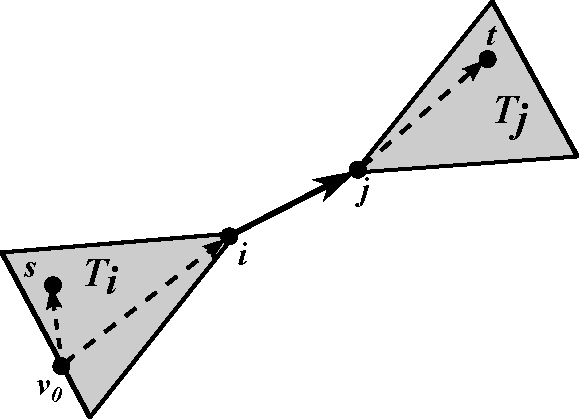
\includegraphics[height=1.2in]{transf_a}
%        \caption{}
%       \label{fig:transf_a}
%   \end{subfigure}%
%    \begin{subfigure}[b]{0.5\textwidth}
%        \centering
%        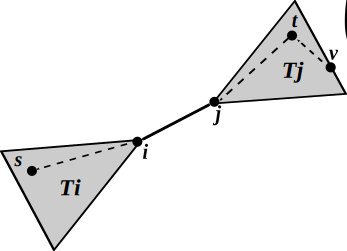
\includegraphics[height=1.2in]{transf_b}
%        \caption{}
%                \label{fig:transf_b}
%    \end{subfigure}
%    \caption{Explanation of the transformations (\ref{eq:tr:fstij}) - (\ref{eq:tr:zij})}
%    \label{fig:transexp}
%\end{figure*}

%In the transformation (\ref{eq:tr:xijj}) of $x_{ij}^s$, we distinguish the situation when $v_0$ and $s$ are in the same subtree, in which case none of the arcs $(i,j)$ and $(j,i)$ carries a flow to $s$, and when $s$ and $v_0$ belong to different subtrees, and there is a flow via $(j,i)$ towards $s$. Again, the last equality is justified since $f_{ij}^s=1\Rightarrow x_{ij}=1$. The relation (\ref{eq:tr:zij}) is obvious.

Having this transformation in hand, it is easy to construct a SMT model based on the minimum Steiner tree model PF1:

    \begin{subequations}
    \begin{flalign}
  \min &  \sum\limits_{(i,j) \in A} \sum\limits_{s \in D_0} p_{ij} y^s_{ij}    \\  \notag  
		   \text{s.t.}&                  && \\	\ 
\label{con:pf1:xfrel}  f^{t}_{ij}   &\leq x_{ij}    ~~ \qquad \qquad t\in D, (i,j)\in A \\
 \label{con:pf1:flow}  \sum\limits_{\substack{ j \in V_i }}f^{t}_{ji}-\sum\limits_{\substack{j\in V_i}}f^{t}_{ij}    & = \begin{cases}
    1~~~~&  t\in D, t = i \\        0~~~~ \qquad             & t\in D_0, i\in V\setminus \{v_0, t\}\end{cases}     \\	
%\label{con:pf2:flowSource}  \sum\limits_{\substack{ j \in V_i }}\check{f}^{st}_{ji}-\sum\limits_{\substack{j\in V_i}}\check{f}^{st}_{ij}    & \geq \begin{cases}
%    -1~~~&  \{s,t\}\in S_0, i = v_0 \\        0  ~~~~   \qquad    & \{s,t\}\in S_0, i\in V\setminus \{v_0\}\end{cases}     \\			
%\label{con:pf2:hookImpFs}  \check{f}^{st}_{ij}    & \leq f^s_{ij}~~   \qquad  \qquad \{s,t\}\in S_0, (i,j)\in A \\	
%\label{con:pf2:hookImpFt}  \check{f}^{st}_{ij}    & \leq f^t_{ij}~~   \qquad    \qquad \{s,t\}\in S_0, (i,j)\in A \\			 		
% \label{con:pf2:stronger}  f^{s}_{ij}+f^{t}_{ij}-\check{f}^{st}_{ij}    &\leq x_{ij}    ~~ \qquad \qquad  \{s,t\}\in S_0, (i,j)\in A \\			 
 \label{con:pf1:flowX}  \sum\limits_{\substack{ j\in V_i }}x_{ji}-\sum\limits_{\substack{j\in V_i}}x_{ij}    & \leq 0~~~~    \qquad\qquad			  i\in V\setminus D \\			 			   	
		  \label{con:pf1:yvar} x_{ij} -f^t_{ij}+f^t_{ji}  &\leq \sum\limits_{\substack{k\in V: \\ p_{ik}\geq p_{ij}}}y^t_{ik}   ~~\quad  t\in D, (i,j)\in A \\  		
\label{con:pf1:B}  \sum_{j\in V_i}x_{ji}&\leq 1~~~~ \qquad  \qquad i\in V\setminus D\\
\label{con:pf1:noflowFromT} f_{ti}^t&=0 ~~~~ \qquad  \qquad t\in D_0, i\in V_t   \\
\label{con:pf1:fitt=xit} f_{it}^t&=x_{it} ~~ \qquad  \qquad t\in D_0, i\in V_t \\
\label{con:pf1:xi0=0} x_{i0}&=0 ~~~~ \qquad  \qquad i\in V_0 \\
\label{con:pf1:fi0s=0} f_{i0}^t&=0 ~~~~ \qquad  \qquad i\in V_0, t\in D \\
\label{con:pf1:fij0=0} f_{ij}^0&=0 ~~~~ \qquad  \qquad (i,j)\in A \\	   			  \label{con:pf1:dim}	\mathbf{x} \in \{0,1\}^{A},\mathbf{f}&\in\{0,1\}^{A \times D_0} \\ 
\label{con:pf1:dimy} \mathbf{y}&\in \{0,1\}^{A\times D}
    \end{flalign}~
    \end{subequations}
    
    Constraints (\ref{con:pf1:flow})-(\ref{con:pf1:flowX}) together with (\ref{con:pf2:dim}) imply that $\mathbf{x}$ induces and arborescence spannind $D$ with node $v_0$ as the root. The constraint (\ref{con:pf1:yvar}) has the same purpose as (\ref{con:dd:yvar}), and is expressed in SMTPF2 space using transformation (\ref{eq:tr:xijj}). Note that the $y_{ij}^s$-variables determining power levels are defined for all destinations $s\in D$, while in the PF2 model of Steiner minimum tree problem, the $f_{ij}^s$ variables are defined only for $s\in D_0$. This inconsistency is resolved by extending the domain of PF2 variables and fixing the newly introduced variables to zero, which is ensured by constraints (\ref{con:pf1:fi0s=0})-(\ref{con:pf1:fij0=0}).
\begin{figure}[!htb]
    \centering
    \begin{subfigure}[b]{0.4\textwidth}
        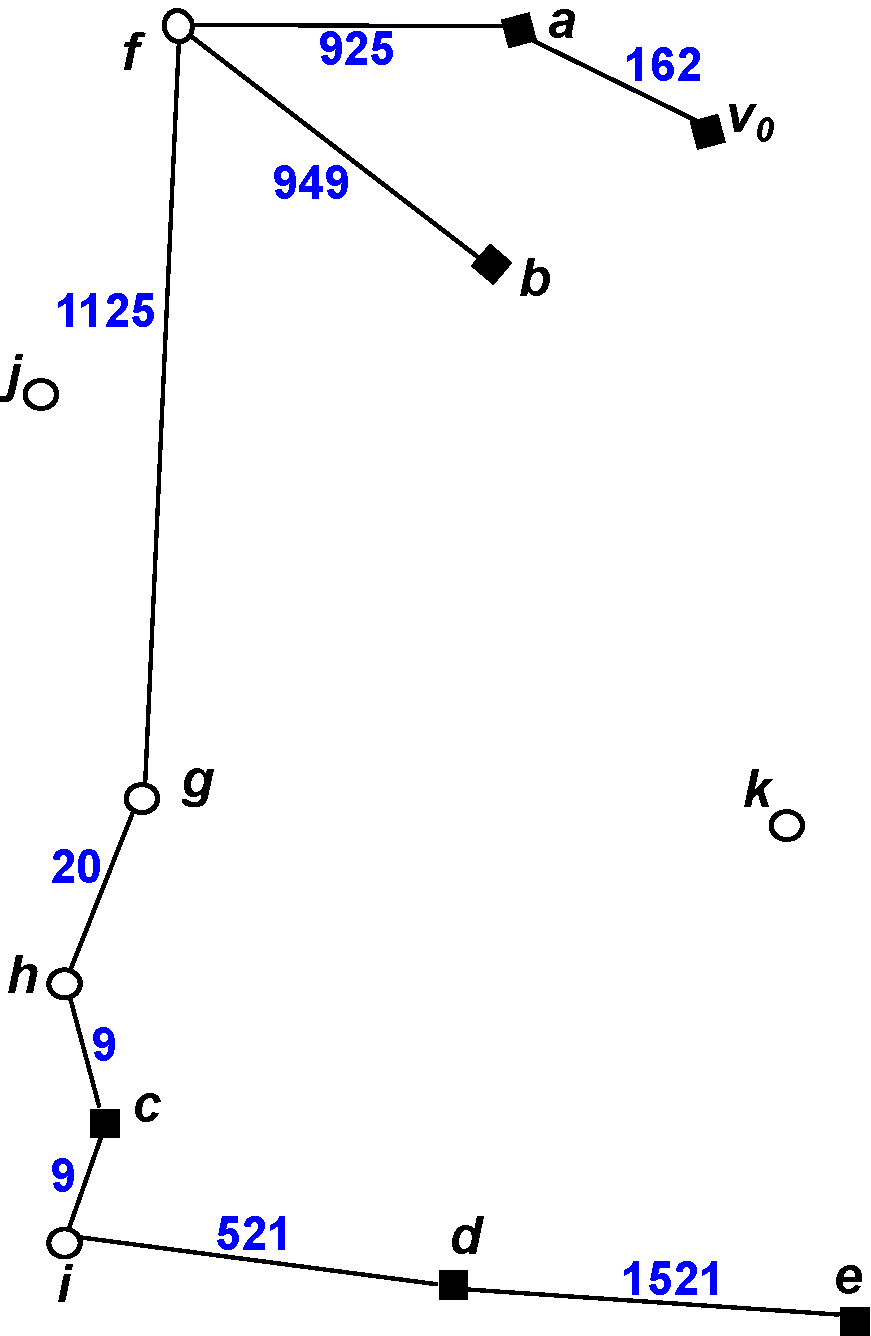
\includegraphics[width=\textwidth]{conBNec}
        \caption{Optimal solution obtained by SMTO. The $z$-variables inducing the resulting tree in this model represent undirected edges. The objective value of this tree is 25156.}
        \label{fig:BorigSMT}
    \end{subfigure}
    \hfill %add desired spacing between images, e. g. ~, \quad, \qquad, \hfill etc. 
      %(or a blank line to force the subfigure onto a new line)
    \begin{subfigure}[b]{0.4\textwidth}
        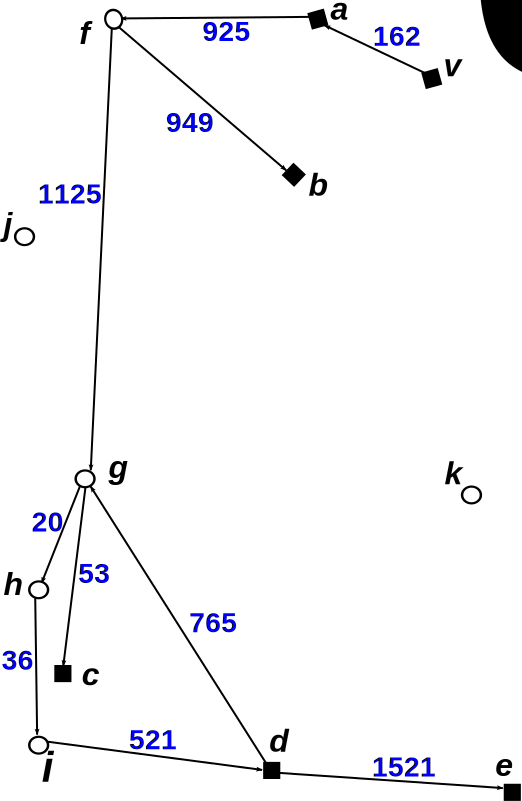
\includegraphics[width=\textwidth]{conBNec2}
        \caption{Solution obtained by SMTPF2 without constraint \ref{con:pf2:B} with objective value 25148. The nodes are connected by arrows because the tree yielded by this model is rooted in a predefined source $v_0$.}
        \label{fig:Bpf2}
    \end{subfigure}
    \caption{An exemplary instance showing why the constraint (\ref{con:pf2:B}) is necessary in SMTPF2. Blue numbers denote power requuirements of connection between nodes. For better legibility, the distances of the links are not proportional.} \label{fig:BProof}
\end{figure}   
     By (\ref{con:pf1:B}) we prevent a non-destination from having multiple entering arcs. This is not necessary in the Steiner minimum tree problem formulation, because the objective function causes, that such solutions are filtered out by optimality. The necessity of this constraint in SMT is demonstrated in Fig. \ref{fig:BProof}. The optimal solution with objective value 25156 to the depicted instance obtained by solving SMTO is shown in Fig. \ref{fig:BorigSMT}. The solution in Fig \ref{fig:Bpf2} yielded by solving SMTPF1 without the constraint (\ref{con:pf1:B}) has objective value 25148, but is clearly not a feasible solution to this instance because of the cycle $(g,h,i,d,g)$. The non-existence of such cycle in a solution given by SMTO model is ensured by constraints (\ref{con:dd:arrowFromDest}), (\ref{con:dd:arrowFromNonDestB}) and (\ref{con:dd:oneDir})\footnote{See detailed proof in \cite{ivanova16isco}}. A transmission commenced in node $c$ is sent via arc $(g,f)$. As a consequence of the link between $g$ and $d$ in Fig. \ref{fig:Bpf2}, the node $d$ also receives the message. This link is absent in Fig. \ref{fig:BorigSMT}, and so $i$ has to relay the signal using the arc $(i,d)$, causing the higher total objective value. Similarly, obvious valid inequalities (\ref{con:pf1:noflowFromT})-(\ref{con:pf1:xi0=0}) are not necessary in the minimum Steiner tree formulation, but are included in order to strengthen the model.
   
\subsection{PF2 Extension [SMTPF2]}
Similarly to the extension of SMTO by the $s-t$-flow variables, the SMTPF1 model can also be extended by 4-index variables. Authors in \cite{Polzin} use variables

%\newline\newline  
  $\check{f}^{st}_{ij}=
	\begin{cases}
    1 & \text{if arc $(i,j) \in A$ carries flow from $v_0$ to both $s$ and $t$, $\{s,t\}\in S_0$},\\
    0 & \text{otherwise},
  \end{cases}$
  describing the common flow from $v_0$ to $s$ and $t$. This allows to create an extended model PF2 by adding constraints relating to the $\check{f}^{st}_{ij}$-variables. An SMT model SMTPF2 based on PF2 has the following form:
 
    \begin{subequations}
    \begin{flalign}
  \min &  \sum\limits_{(i,j) \in A} \sum\limits_{s \in D} p_{ij} y^s_{ij}    \\  \notag  
		   \text{s.t.}&                  && \\			   
		   (\ref{con:pf1:flow}) - (\ref{con:pf1:fij0=0}) \notag \\ 	
\label{con:pf2:flowHook}  \sum\limits_{\substack{ j \in V_i }}\check{f}^{st}_{ji}-\sum\limits_{\substack{j\in V_i}}\check{f}^{st}_{ij}    & \geq \begin{cases}
    -1~~~&  \{s,t\}\in \check{S_0}, i = 0 \\        0  ~~~~   \qquad         & \{s,t\}\in \check{S_0}, i\in V\setminus \{v_0\}\end{cases}     \\			
\label{con:pf2:startInSource}  \check{f}^{st}_{ij}    & \leq f^s_{ij}~~   \qquad  \qquad \{s,t\}\in \check{S_0}, (i,j)\in A \\	
\label{con:pf2:stopInDest}  \check{f}^{st}_{ij}    & \leq f^t_{ij}~~   \qquad    \qquad \{s,t\}\in \check{S_0}, (i,j)\in A \\			 		
 \label{con:pf2:stronger}  f^{s}_{ij}+f^{t}_{ij}-\check{f}^{st}_{ij}    &\leq x_{ij}    ~~ \qquad \qquad  \{s,t\}\in \check{S_0}, (i,j)\in A \\			 	   			  
 \label{con:pf2:dim}  \mathbf{x}     \in \{0,1\}^A,  \mathbf{f}&\in \{0,1\}^{A\times D}, \mathbf{\check{f}}\in\{0,1\}^{A\times \check{S_0}}\\
 \label{con:pf2:dim2}  \mathbf{y} & \in \{0,1\}^{A\times D}
    \end{flalign}~
    \end{subequations}

By (\ref{con:pf2:flowHook}) is ensured that the common flow is non-increasing. The inequalities (\ref{con:pf2:stronger}) replace a weaker (\ref{con:pf1:xfrel}).

\section{Constraint Generation}
The stronger SMT models SMTMF and SMTPF2 are too large and are therefore not very practical for solving even fairly small instances.  The main idea of how to make this model more useful in practice is to solve a relaxation of the model where some of the constraints are omitted. Relaxed constraints that are violated in the obtained solutions can be dynamically  added to the model and the whole process is repeated. This approach is known as \emph{constraint generation scheme}.

\subsection{SMTMF}
First, we relax the flow constraints, which means that we solve only SMTO-LP. This gives the vector $\mathbf{x}$, which, by constraint (\ref{con:mf:fcap}), acts as a capacity vector, and determines the maximum possible amount of flow through certain arc. We then go through all possible $s-t$ pairs of destinations and check whether the flow constraints are fulfilled for the particular $s$ and $t$. This is equivalent to solving a maximum flow problem, and those $s-t$-pairs for which there is no feasible solution are stored. After all pairs are processed, new flow constraints for some (possibly all) stored $s-t$-pairs are added to the model, and the whole process is repeated until there are no violated flow constraints for any $s-t$ pair. The algorithm \ref{alg:congen} describes this process more formally.

There are various strategies how to determine which of the violated flow constraints will be added to the model. 

\section{Transformations and Valid Inequalities}

In order to create a SMTPF1 model, it was necessary to express $x^s_{ij}$ variables in PF1 space using relation (\ref{eq:tr:xijj1}). The aim of this section is to show, how the entire SMTMF model can be converted into an equivalent model that uses only variables of SMTPF2. 

The following equations express all variables from SMTMF in SMTPF2 space:
\begin{subequations}
\begin{align}
\notag\label{eq:tr:fstij}f^{st}_{ij}&=f^t_{ij}(1-\check{f}^{st}_{ij})+f^{s}_{ji}(1-\check{f}^{st}_{ji})= \\
&=  f^t_{ij}+f^s_{ji} - \check{f}^{st}_{ij} - \check{f}^{st}_{ji}& (i,j)\in A, \{s,t\}\in S_0\\
\notag\label{eq:tr:xijj}x^s_{ij}&=x_{ij}(1-f^{s}_{ij})(1-f^{s}_{ji})+x_{ji}f^{s}_{ji}=
\\&= x_{ij}-f^s_{ij} + f^{s}_{ji} & (i,j)\in A, s\in D_0\\
\label{eq:tr:zij}z_{ij}&=x_{ij}+x_{ji}& \{i,j\}\in E
\end{align}
\end{subequations}

Let $T=(V_T,E_T)$ be a multicast tree, and consider an edge $\{i,j\}\in E_T$ dividing $T$ into two subtrees $T_i$ and $T_j$ rooted in $i$ and $j$, respectively.  If the arc $(i,j)$ caries and $s-t$-flow from $s\in D$ to $t\in D$, then $s$ and $t$ must lie in different subtrees. Node $v_0$ lies either in $T_i$ or $T_j$.
%as depicted in Fig. \ref{fig:transf_a} and Fig. \ref{fig:transf_b}, respectively.
These two cases are captured by the first equality in (\ref{eq:tr:fstij}). If both $v_0$ and $s$ lie in $T_i$, then $f_{ij}^t=1$. Similarly, if $v_0$ and $t$ lie in $T_j$, then $f_{ji}^s=1$. The expressions in parentheses prevent $s$ and $t$ belonging to the same subtree. Using the implications $\check{f^{st}_{ij}}=1\Rightarrow f_{ij}^t=1$ and $\check{f^{st}_{ji}}=1\Rightarrow f_{ji}^s=1$ that follow from the interpretation of variables, we justify the second equality expressing this relation linearly.
%\begin{figure*}[h!]
%    \centering
%    \begin{subfigure}[b]{0.5\textwidth}
%       \centering
%      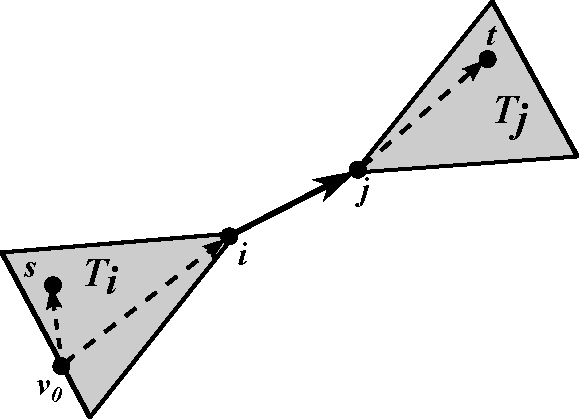
\includegraphics[height=1.2in]{transf_a}
%        \caption{}
%       \label{fig:transf_a}
%   \end{subfigure}%
%    \begin{subfigure}[b]{0.5\textwidth}
%        \centering
%        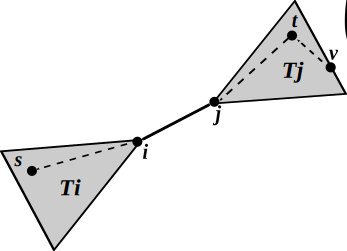
\includegraphics[height=1.2in]{transf_b}
%        \caption{}                \label{fig:transf_b}
%    \end{subfigure}
%    \caption{Explanation of the transformations (\ref{eq:tr:fstij}) - (\ref{eq:tr:zij})}
%    \label{fig:transexp}
%\end{figure*}
In the transformation (\ref{eq:tr:xijj}) of $x_{ij}^s$, we distinguish the situation when $v_0$ and $s$ are in the same subtree, in which case none of the arcs $(i,j)$ and $(j,i)$ carries a flow to $s$, and when $s$ and $v_0$ belong to different subtrees, and there is a flow via $(j,i)$ towards $s$. Again, the last equality is justified since $f_{ij}^s=1\Rightarrow x_{ij}=1$. The relation (\ref{eq:tr:zij}) is obvious.

By a similar approach, we achieve the transformation from SMTMF space to PF2 space. 
\begin{subequations}
\begin{align}
\label{eq:tr:fstij2}x_{ij}=&x^0_{ij} & (i,j)\in A\\
\label{eq:tr:fijt2}f^t_{ij}=&x^t_{ji}x^0_{ij}=f^{0t}_{ij} & (i,j)\in A, t\in D_0\\
\label{eq:tr:fstij2}\check{f}^{st}_{ij}=& x^s_{ji}x^t_{ji}x^0_{ij} & (i,j)\in A, \{s,t\}\in S_0
\end{align}
\end{subequations}

We aim to compare the models presented in Section \ref{sec:ILP} in terms of strength. The results obtained by numerical experiments presented in the next section suggest, that PF2 model is stronger than SMTMF. This section attempts to prove this conjecture. First, we express the SMTMF model in PF2 space using transformations (\ref{eq:tr:fstij})-(\ref{eq:tr:zij}). This formulation is referred to as MF-PF2.

 	\begin{small} 	
\begin{subequations}
\begin{flalign}
\label{objective:mfinpf2} &\makebox[0pt][l]{$\displaystyle{}\min \sum\limits_{(i,j) \in A} \sum\limits_{s \in D} p_{ij} y^s_{ij} $}  & &&\\ \notag  
   \text{s.t.}&  &  &                 && \\	\
\label{con:mfinpf2:maxsize}   \sum\limits_{\{i,j\}\in E}(x_{ij}+x_{ji}) & \leq  N-1  &   && \\
     \label{con:mfinpf2:arrowFromDest}  \sum\limits_{j\in V_i}(x_{ji}-f^s_{ji}+f^s_{ij})          & = 1       			&& i\in D, s\in D_0, i \neq s && \\ 
		  \label{con:mfinpf2:arrowFromNonDestB}  \sum\limits_{j \in V_i}(x_{ji}-f^s_{ji}+f^s_{ij})  &\leq 1 && i\in V \setminus D, s\in D_0   &&\\		
		  \label{con:mfinpf2:arrowFromNonDestA}  x_{ik}-f^s_{ik}+f^s_{ki}  & \leq \sum\limits_{j \in V_i\setminus\{k\}}(x_{ji}-f^s_{ji}+f^s_{ij}) &&
		  i\in V \setminus D,k\in V_i, s\in D_0   &&\\		  
      \label{con:mfinpf2:extraCon}  \sum\limits_{j \in V_i}(x_{ji}-f^s_{ji}+f^s_{ij}) & \leq \sum\limits_{j \in V_i}(x_{kj}-f^s_{kj}+f^s_{jk}) &&  i\in V\setminus D, s\in D_0  &&\\			  \label{con:mfinpf2:startInSource}  x_{js} - f^s_{js}+f^s_{sj}    & = 0       			&&  s\in D_0, j\in V_s &&\\		 
		  \label{con:mfinpf2:yvar}  x_{ij}-f^s_{ij}+f^s_{ji} & \leq \sum\limits_{k\in V:p_{ik}\geq p_{ij}}y^s_{ik} && s\in D_0, (i,j)\in A 		&&\\  
		 		 \label{con:mfinpf2:flowNormal}  \sum\limits_{\substack{ j\in V_i }}f^t_{ij}-\sum\limits_{\substack{j\in V_i }}f^t_{ji}    & = 0     			&& i\in V, t\in D_0, i \neq t &&\\	
		 	 \label{con:mfinpf2:flowDest}  \sum\limits_{\substack{j\in V_t}}f^t_{tj}-\sum\limits_{\substack{j\in V_t}}f^t_{jt}    & = -1     			&&  t \in D_0 &&\\	
%		 			 	 \label{con:mfinpf2:flowSource}  \sum\limits_{\substack{ (s,j)\in A}}(f^t_{sj}+f^s_{js})-\sum\limits_{\substack{(j,s)\in A}}(f^t_{js}+f^s_{sj})    & = 1     			&&  \{s,t\}\subseteq D_0 && \\	
           \label{con:mfinpf2:fcap}   f^t_{ij} - \check{f}^{st}_{ij} - \check{f}^{st}_{ji} &\leq  x_{ij}-f^s_{ij}   && (i,j)\in A, \{s,t\}\in S_0 && &\\ 		 			 	 
		    \label{con:mfinpf2:zbound} x_{ij}+x_{ji}&\leq 1 &&\{i,j\}\in E \\
  		    \label{con:mfinpf2:xbound} 0\leq x_{ij}-f_{ij}^s+f_{ji}^s & \leq 1 && \{i,j\}\in E,  s\in D_0 \\
\label{con:mfinpf2:fbound} 0\leq f_{ij}^t+f_{ji}^s-\check{f}_{ij}^{st}-\check{f}_{ji}^{st} & \leq 1 && \{i,j\}\in E,\{s,t\}\in D_0 \\
(\ref{con:pf1:xi0=0}) - (\ref{con:pf1:fij0=0}) \notag \\ 
		    \label{con:mfinpf2:dim}	\mathbf{x} \in \{0,1\}^{A},\mathbf{f}&\in\{0,1\}^{A \times D_0},\mathbf{\check{f}}\in\{0,1\}^{A\times S_0} \\ 
		    \label{con:mfinpf2:dimy}\mathbf{y}&\in \{0,1\}^{A\times D}
    \end{flalign}
    \end{subequations}  
\end{small}

Note that the 4-index variables $\check{f}^{st}_{ij}$ appear only in (\ref{con:mfinpf2:fcap}) and (\ref{con:mfinpf2:fbound}). Assigning the highest possible values $\check{f}^{st}_{ij}=f^{t}_{ij}$ and $\check{f}^{st}_{ji}=f^{s}_{ji}$ according to (\ref{con:mfinpf2:fbound}) does not cause a violation of any other constraint. It is therefore possible to remove (\ref{con:mfinpf2:fcap}) and (\ref{con:mfinpf2:fbound}) resulting in a model in SMTPF1 space (with up to 3-index variables) equivalent to the SMTMF model. 

We now analyze whether all solutions satisfying an LP relaxation of (\ref{con:pf1:xfrel})-(\ref{con:pf1:dimy}) satisfy (\ref{con:mfinpf2:maxsize})-(\ref{con:mfinpf2:dimy}), also with relaxed integrality constraints. First, we prove that they satisfy:
\begin{align*}
\sum_{j\in V_i}x_{ji}&=1,~~~~~~ i\in D_1, & \label{eq:sumToD} \tag{A}\\
%f_{ij}^t&\leq x_{ij},~~~~ (i,j)\in A, t\in D_1. & \label{eq:fimpx} \tag{B} \\
\end{align*}
%\sum_{j\in V_i^-}x_{ji}&\leq 1,~~~~~~ i\in V\setminus D, &(B)\\


\begin{itemize}

\item[](\ref{eq:sumToD}): Utilizing first (\ref{con:pf1:fitt=xit}), next (\ref{con:pf1:flow}) for $t=i$, and finally (\ref{con:pf1:noflowFromT}), we get
$$\sum_{j\in V_i}x_{ji}=\sum_{j\in V_i}f_{ji}^i = 1+\sum_{j\in V_i}f_{ij}^i=1.$$

\item[] (\ref{con:mfinpf2:maxsize}): Follows directly from (\ref{eq:sumToD}) and (\ref{con:pf1:B}).

\item[] (\ref{con:mfinpf2:arrowFromDest}): Assume $t\in D_1$ and $i\in D_1\setminus\{t\}$. Flow conservation (\ref{con:pf1:flow}) implies
$$\sum_{j\in V_i}x_{ji} - \sum_{j\in V_i}f_{ji}^t + \sum_{j\in V_i}f_{ij}^t = \sum_{j\in V_i}x_{ji}.$$ Then (\ref{con:mfinpf2:arrowFromDest}) follows from (\ref{eq:sumToD}).
Assume $i=v_0$: Due to (\ref{con:pf1:xi0=0}) and (\ref{con:pf1:fi0s=0}), the first two sums equal to zero, which gives
$$\sum_{j\in V_i}x_{ji} - \sum_{j\in V_i}f_{ji}^t + \sum_{j\in V_i}f_{ij}^t = \sum_{j\in V_i}f_{ij}^t = 1,$$
where the latter equality follows by summing (\ref{con:pf1:flow}) over all $i\in V\setminus\{v_0\}$.

\item[] (\ref{con:mfinpf2:arrowFromNonDestB}): The proof is analogous to (\ref{con:mfinpf2:arrowFromDest}), with (\ref{con:pf1:B}) replacing (\ref{eq:sumToD}).
%\item[] (\ref{con:mfinpf2:arrowFromNonDestB}): Proof missing.

\item[] (\ref{con:mfinpf2:extraCon}): Follows immediately from (\ref{con:pf1:flowX}) by utilizing flow conservation (\ref{con:pf1:flow}) at node $j$.

\item[] (\ref{con:mfinpf2:startInSource}): Follows from (\ref{con:pf1:noflowFromT}) and (\ref{con:pf1:fitt=xit}).

\item[] (\ref{con:mfinpf2:yvar}): Follows from (\ref{con:pf1:yvar}).

\item[] (\ref{con:mfinpf2:flowNormal})-(\ref{con:mfinpf2:flowDest}): All four-index variables cancel out. Thus, (\ref{con:mfinpf2:flowNormal}) follows from flow conservation (\ref{con:pf1:flow}) at $i$.

%\item[] (\ref{con:mfinpf2:fcap}): Follows from (\ref{con:pf2:stronger}).


%\item[] (\ref{con:mfinpf2:zbound}): Failed attempt: Assume $x_{ij}+x_{ji}>1$ for some $\{i,j\}\in E$. Then, there exists $s\in D_1$ such that $f^s_{ij}=x_{ij}$ and by flow conservation, $\sum_{k\in V^-_{i}}f^s_{ki}\geq f^s_{ij}=x_{ij}.$ Now we distinguish two cases: 1) If $f^s_{ji}=0$, then there is some $s_1\neq s$ such that $f^{s_1}_{ji}+f^s_{ij}>1.$ But then also 
%$$\sum_{k\in V^-_{i}\setminus\{j\}}f^s_{ki}+f^{s_1}_{ji}>1\Rightarrow\sum_{k\in V^-_{i}\setminus\{j\}}x_{ki}+x_{ji}>1\Rightarrow\sum_{k\in V^-_{i}}x_{ki}>1,$$
%contradicting either (\ref{eq:sumToD}), if $i\in D_1$, or (\ref{con:pf2:B}), if $i\in V\setminus D$. 2) If $f^s_{ji}>0$, a flow of size $\min\{f^s_{ij},f^s_{ji}\}$ can be sent in a reverse direction leading to a solution that is no worse than the original one.

\item[] (\ref{con:mfinpf2:xbound}): The lower bound follows from (\ref{con:pf1:xfrel}). The upper bound follows from (\ref{con:mfinpf2:arrowFromDest}) for $i\in D$ and from (\ref{con:mfinpf2:arrowFromNonDestB}) for $i\in V\setminus D$. To see this, observe that each term in the sums in (\ref{con:mfinpf2:arrowFromDest})-(\ref{con:mfinpf2:arrowFromNonDestB}) is non-negative because of (\ref{con:pf1:xfrel}). 
%\item[] (\ref{con:mfinpf2:fbound}): The lower bound follows from (\ref{con:pf2:hookImpFs})-(\ref{con:pf2:hookImpFt}). From (\ref{eq:fimpx}) and (\ref{con:mfinpf2:zbound}), we get the upper bound
$$f^t_{ij}+f^s_{ji}-f^{st}_{ij}-f^{st}_{ji}\leq f^t_{ij}+f^s_{ji}\leq x_{ij}+x_{ji}\leq 1$$
\end{itemize}
This analysis unfortunately does not prove completely that SMTPF1 implies SMTMF. Constraints (\ref{con:mfinpf2:arrowFromNonDestA}) and (\ref{con:mfinpf2:zbound}) are yet to be proved.  

\subsection{Valid Inequalities}
This SMTMF model can be further extended by valid inequalities strengthening its LP bounds:
  \begin{subequations}
  \begin{flalign}
\label{con:vi:xImpY}  x^{s}_{ij} & \leq \sum\limits_{t\in D\setminus\{s\}}  f^{st}_{ij},  \quad\quad    (i,j)\in A,s\in D \\
 \label{con:vi:Y1}  \sum\limits_{j\in V\setminus\{s\}}  y^{s}_{sj} & =1,  \quad\quad\quad\quad\quad\quad    s\in D \\
\notag\label{con:vi:f2dest}  f^{st_1}_{ij}-f^{st_2}_{ij}+f^{t_1t_2}_{ij} & \geq 0, \quad\quad\quad\quad\quad\quad (i,j) \in A, \\  & \quad\quad\quad\quad\quad\quad\quad\quad(s,t_1),(s,t_2),(t_1,t_2)\in S \\
\label{con:vi:sumYImpSumX} \sum\limits_{i\in V\setminus\{j\} }y^{s}_{ji} & \geq \sum\limits_{i\in V\setminus\{j\}}  x^{s}_{ij},   \quad\quad   j\in V\setminus D, s\in D \\
\label{con:vi:sumFImpSumY} \sum\limits_{i\in V\setminus\{j\}, p_{ji}\geq p_{jk}  }f^{st}_{ji} & \leq \sum\limits_{i\in V\setminus\{j\}, p_{ji}\geq p_{jk}}  y^{s}_{ji},   j,k\in V, (s,t)\in S
\end{flalign}
  \end{subequations}
  
The first valid inequality (\ref{con:vi:xImpY}) expresses that whenever an arc $(i,j)$ carries a signal from $s$, there must be at least one destination other than $s$ receiving it. That means that $(i,j)$ carries an $(s,t)$-flow from $s$ to $t$. The inequality (\ref{con:vi:Y1} says that there has to be exactly one neighbour $j\in V$ of $s\in D$, such that $s$ uses the power $p_{sj}$ in order to transmit its own signal. Signal never disappears in a non-destination. As (\ref{con:vi:sumYImpSumX}) states, if a non-destination $j$ receives a signal from $s$, then there is a node $i\in V$ to whom the signal is forwarded using power $p_{ji}$. Consider nodes $j,k\in V$ and a pair of destinations $(s,t)$. If an $(s,t)$-flow is sent through $(j,i)$ such that $p_{ji}\geq p_{jk}$, then a message from $s$ must be relayed by $j$ using power level at least $p_{jk}$.

It follows from the domain of $\mathbf{\check{f}}$, that 
\begin{equation}
\label{eq:fhooksym}
\check{f}_{ij}^{st}=\check{f}_{ij}^{ts},
\end{equation}
because $S_0$ is a set of 2-element sets. By the implicit assumption of (\ref{eq:fhooksym}) in SMTPF2, it is possible to infer additional valid inequalities for SMTMF. We can also write
\begin{align*}
\check{f}^{st}_{ij}+\check{f}^{st}_{ji}=\check{f}^{ts}_{ij}+\check{f}^{ts}_{ji} &\Rightarrow f^t_{ij}+f^s_{ji}-f^{st}_{ij}=f^s_{ij}+f^t_{ji}-f^{ts}_{ij}\Rightarrow \\ & \Rightarrow f^{0t}_{ij}+f^{0s}_{ji}-f^{st}_{ij}=f^{0s}_{ij}+f^{0t}_{ji}-f^{ts}_{ij}.
\end{align*}
The first and second implication follow from the transformation (\ref{eq:tr:fstij}) and (\ref{eq:tr:fijt2}), respectively. The last equality consists of only variables from SMTMF  space, and so the valid inequality
\begin{equation*}f^{ut}_{ij}+f^{us}_{ji}+f^{ts}_{ij}=f^{us}_{ij}+f^{ut}_{ji}+f^{st}_{ij} \quad\quad (u,t),(u,s),(s,t),(t,s)\in S_0, i,j\in V
\end{equation*} 
can be added to the SMTMF. All the occurances of $v_0$ were replaced by a general destination $u\in D$, because $v_0$ does not have any special role in SMTMF.
 
%From (\ref{con:pf2:hookImpFs}), (\ref{con:pf2:hookImpFt}) and (\ref{eq:tr:fijt2}) we have that $\check{f}^{st}_{ij}\leq f^{0s}_{ij}$ and $\check{f}^{st}_{ij}\leq f^{0t}_{ij}$. Combining these two inequalities yields valid inequalities
%\[
%\left.
%\begin{array}{ll}
%\check{f}^{st}_{ij}+\check{f}^{st}_{ji}&\leq f^{0s}_{ij}+f^{0s}_{ji} \\[.2cm]
%check{f}^{st}_{ij}+\check{f}^{st}_{ji}&\leq f^{0s}_{ij}+f^{0t}_{ji} \\[.2cm]
%\check{f}^{st}_{ij}+\check{f}^{st}_{ji}&\leq f^{0t}_{ij}+f^{0s}_{ji} \\[.2cm]
%\check{f}^{st}_{ij}+\check{f}^{st}_{ji}&\leq f^{0t}_{ij}+f^{0t}_{ji} 
%\end{array}
%\right\} \Rightarrow
%\left\{
%\begin{array}{ll}
%f^{st}_{ij}&\geq f^{0t}_{ij}-f^{0s}_{ij} \\[.2cm]
%f^{st}_{ij}&\geq f^{0t}_{ij}-f^{0s}_{ij} + f^{0s}_{ji} - f^{0t}_{ji} \\[.2cm]
%f^{st}_{ij}&\geq 0 \\[.2cm]
%f^{st}_{ij}&\geq f^{0s}_{ji}-f^{0t}_{ji}
%\end{array}.
%\right.
%\]
%If some of them are not already implied by constraints in SMTMF, the can be included in the model. The implication is justified by (\ref{eq:tr:fstij}) and (\ref{eq:tr:fijt2}).

\section{Experimental Evaluation}
\label{sec:exp}
The practical part of this work focuses on comparison of the models presented in the previous section. As the main focus of this study is to determine tighter bounds, the conducted experiments are designed for this purpose. Instances of intended number of vertices are generated with random coordinates uniformly distributed between [0, 0] and [100, 100]. All computations were made on an Intel Core 2 Quad CPU at 2.83 GHz and 8 GB RAM.


\subsection{Comparison of the models}

In the following experiments, two different scenarios are considered. First, we create instances with constant number of destinations, and the number of non-destinations gradually increases. Conversely, in the second scenario, the number of non-destinations is fixed, while the number of destinations increases. The models are compared with respect to the objective value of their solutions and CPU time.

We compared models SMTO-LP, SMTMF-LP, SMTPF2-LP and SMTO, with results marked in graphs in Fig. \ref{fig:id-basi}. We can clearly see that the SMTMF-LP and SMTPF2-LP are stronger than SMTO-LP, and the difference increases with increasing number of nodes. Nevertheless, the best LP bounds are still far from the integer solution. The difference between SMTMF-LP and SMTPF2-LP seems negligible, however, the latter one is always slightly stronger, in average by 0.33\% for the largest instances. 

The CPU time of the SMTPF2-LP model seems to be more favourable than SMTMF-LP for instances with lower ratio $|V|/|D|$. 
\begin{figure*}[h!]
    \centering
    \begin{subfigure}[b]{0.5\textwidth}
        \centering
        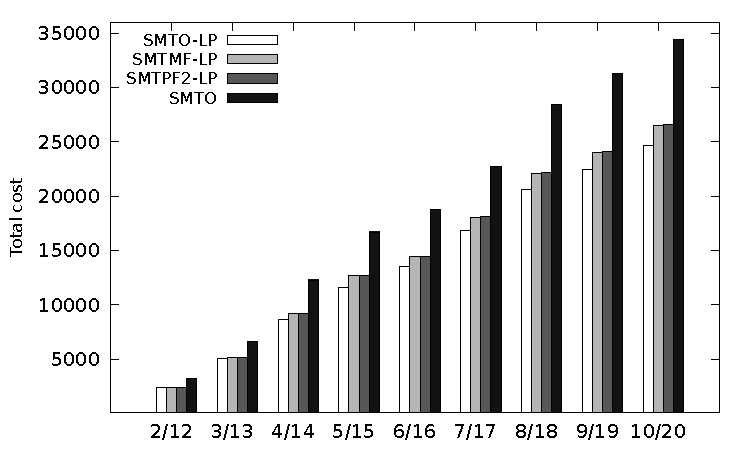
\includegraphics[height=1.2in]{../graphs/id-basic-cost}
        \caption{}
        \label{fig:id-basic-cost}
    \end{subfigure}%
    \begin{subfigure}[b]{0.5\textwidth}
        \centering
        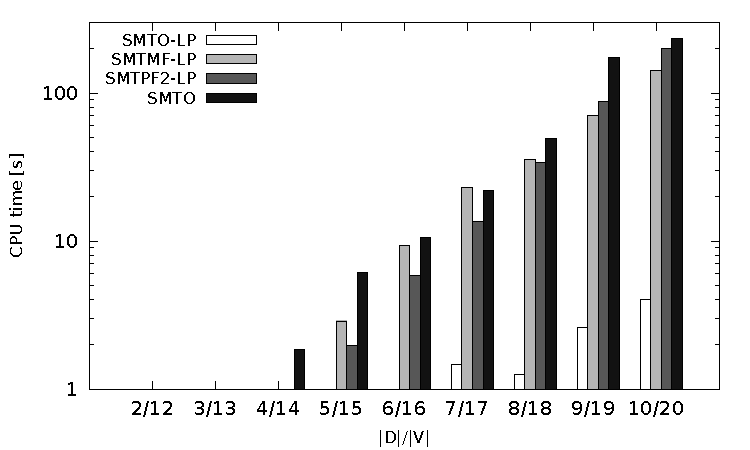
\includegraphics[height=1.2in]{../graphs/id-basic-time}
        \caption{}
                \label{fig:id-basic-time}
    \end{subfigure}
    \caption{}
    \label{fig:id-basi}
\end{figure*}


\begin{figure*}[h!]
    \centering
    \begin{subfigure}[b]{0.5\textwidth}
        \centering
        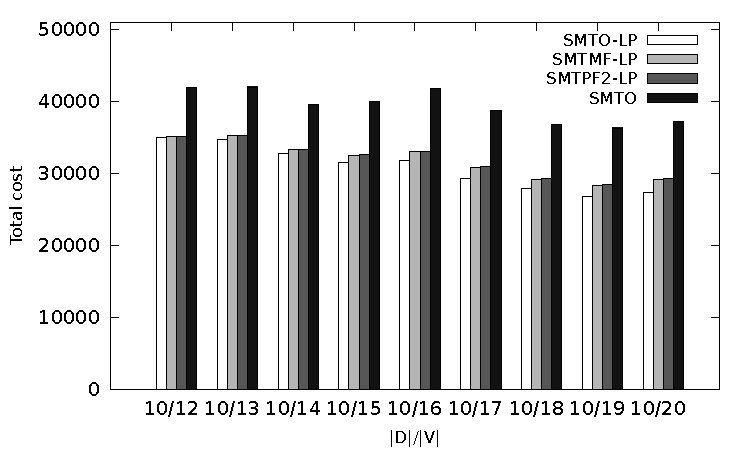
\includegraphics[height=1.2in]{../graphs/in-basic-cost}
        \caption{}
        \label{fig:in-basic-cost}
    \end{subfigure}%
    \begin{subfigure}[b]{0.5\textwidth}
        \centering
        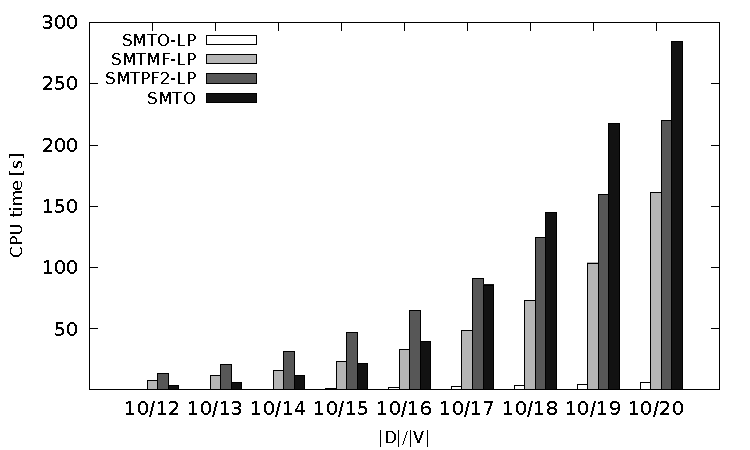
\includegraphics[height=1.2in]{../graphs/in-basic-time}
        \caption{}
                \label{fig:in-basic-time}
    \end{subfigure}
    \caption{}
    \label{fig:in-basic}
\end{figure*}


\section{Conclusion and Future Work}
\label{sec:conclusion}
%as required. Don't forget to give each section
%and subsection a unique label (see Sect.~\ref{sec:1}).
%\paragraph{Paragraph headings} Use paragraph headings as needed.
%\begin{equation}
%a^2+b^2=c^2
%\end{equation}

% For one-column wide figures use
%\begin{figure}
% Use the relevant command to insert your figure file.
% For example, with the graphicx package use
%  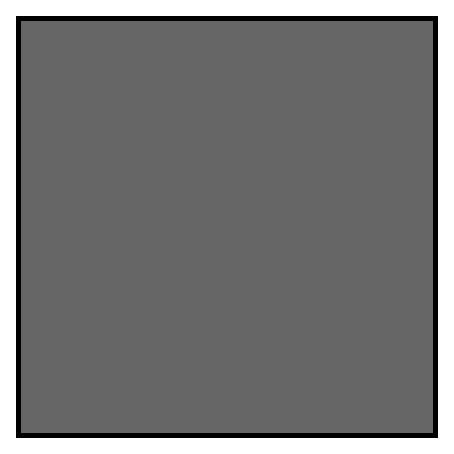
\includegraphics{example.eps}
% figure caption is below the figure
%\caption{Please write your figure caption here}
%\label{fig:1}       % Give a unique label
%\end{figure}
%
% For two-column wide figures use
%\begin{figure*}
% Use the relevant command to insert your figure file.
% For example, with the graphicx package use
%  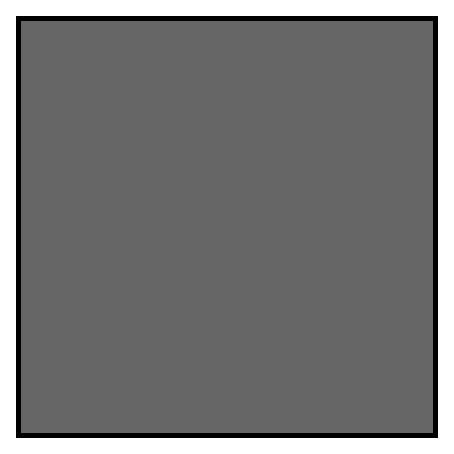
\includegraphics[width=0.75\textwidth]{example.eps}
% figure caption is below the figure
%\caption{Please write your figure caption here}
%\label{fig:2}       % Give a unique label
%\end{figure*}
%
% For tables use
%\begin{table}
% table caption is above the table
%\caption{Please write your table caption here}
%\label{tab:1}       % Give a unique label
% For LaTeX tables use
%\begin{tabular}{lll}
%\hline\noalign{\smallskip}
%first & second & third  \\
%\noalign{\smallskip}\hline\noalign{\smallskip}
%number & number & number \\
%number & number & number \\
%\noalign{\smallskip}\hline
%\end{tabular}
%\end{table}


%\begin{acknowledgements}
%If you'd like to thank anyone, place your comments here
%and remove the percent signs.
%\end{acknowledgements}

% BibTeX users please use one of
%\bibliographystyle{spbasic}      % basic style, author-year citations
%\bibliographystyle{spmpsci}      % mathematics and physical sciences
%\bibliographystyle{spphys}       % APS-like style for physics
%\bibliography{}   % name your BibTeX data base

% Non-BibTeX users please use
\begin{thebibliography}{}
%
% and use \bibitem to create references. Consult the Instructions
% for authors for reference list style.
%
\bibitem{Wieseltier00onthe}
Wieselthier,  J. E., Nguyen, G. D., Ephremides, A.,
On the Construction of Energy-Efficient Broadcast and Multicast Trees in Wireless Networks,
Proceedings of the Nineteenth Annual Joint Conference of the IEEE Computer and Communications Societies.
2, 585--594 (2000)

\bibitem{Haugland12Dual}
Yuan, D., Haugland, D.,
Dual Decomposition for Computational Optimization of Minimum-Power Shared Broadcast Tree in Wireless Networks,
IEEE Transactions on Mobile Computing,
12, 11, 2008--2019 (2012)

\bibitem{Polzin}
Polzin, T., Daneshmand, S. V., A comparison of Steiner tree relaxations, Discrete Applied Mathematics, 112,  1-3, 15 241--261, (2001)

\bibitem{ivanova16isco}
Ivanova, M., Shared Multicast Trees in Ad Hoc Wireless Networks, Combinatorial Optimization, 4th International Symposium, ISCO 2016, 241--261, (2016)

\bibitem{Haugland11Compact}
Haugland, D., Yuan, D.,
Wireless Network Design: Optimization Models and Solution Procedure, 219--246,
International Series in Operations Research \& Management Science.
Springer, New York, (2011)

%\bibitem{RefJ}
% Format for Journal Reference
%Author, Article title, Journal, Volume, page numbers (year)
% Format for books
%\bibitem{RefB}
%Author, Book title, page numbers. Publisher, place (year)
% etc
\end{thebibliography}

\end{document}
% end of file template.tex

